\documentclass[14pt]{extarticle}
\usepackage{cmap}
\usepackage[T2A]{fontenc}
\usepackage[utf8]{inputenc}
\usepackage[russian]{babel}
\usepackage[a4paper, left=25mm, right=15mm, top=20mm, bottom=20mm]{geometry}
\usepackage{amsmath, amssymb}
\usepackage{graphicx}
\usepackage{float}
\usepackage{booktabs}
\usepackage{array}
\usepackage{caption}
\usepackage{indentfirst}
\usepackage{enumitem}
\usepackage[hidelinks]{hyperref}
\usepackage{setspace}

\graphicspath{{figures/}}
\captionsetup{labelsep=period, font=small}
\captionsetup[table]{justification=raggedleft, singlelinecheck=false}
\setlength{\parindent}{1.25cm}
\onehalfspacing
\setlist{nosep, leftmargin=1.5cm}
\renewcommand{\arraystretch}{1.12}
\newcommand{\nm}[1]{\overline{#1}}

% ---------- титульный лист ----------
% #1 -- номер работы, #2 -- тема
\newcommand{\itmotitle}[2]{%
\begin{titlepage}
\begin{center}
\singlespacing
Министерство науки и высшего образования Российской Федерации\\[2mm]
Федеральное государственное автономное образовательное учреждение высшего образования
«Национальный исследовательский университет ИТМО»\\
(университет ИТМО)\\[6mm]
Факультет «Систем управления и робототехники»

\vspace{38mm}

{\large\bfseries ОТЧЕТ\\[1mm] О ЛАБОРАТОРНОЙ РАБОТЕ №#1}\\[4mm]
По дисциплине «Электроника и схемотехника»\\[3mm]
на тему:\\[1mm]
{\bfseries «#2»}\\[6mm]
Вариант 2
\end{center}

\vspace{30mm}

\begin{flushright}
\begin{minipage}{0.62\textwidth}
\singlespacing
Преподаватель: Зарина Ольга Андреевна\\[4mm]
Выполнили:\\
Басиони Адельсалам Али Абдельсалам -- 465144\\
Боврджи Тамим Махер Мохаммед -- 412894\\[4mm]
Поток: ЭЛЕК И СХЕМ R БАК 1.2
\end{minipage}
\end{flushright}

\vfill
\begin{center}
г. Санкт-Петербург\\
2026
\end{center}
\end{titlepage}
\setcounter{page}{2}
}


\begin{document}
\itmotitle{7.1}{Комбинационные логические элементы: мультиплексоры, демультиплексоры, шифраторы, дешифраторы, сумматоры}

\tableofcontents
\newpage

\section*{Цель работы}
\addcontentsline{toc}{section}{Цель работы}
Собрать и исследовать работу базовых комбинационных логических схем: мультиплексора,
демультиплексора, шифратора (кодера), дешифратора (декодера) и двоичного сумматора.
Выполнить моделирование в LTspice, построить таблицы истинности, проанализировать работу
схем при всех возможных комбинациях входов.

\section*{Исходные данные}
\addcontentsline{toc}{section}{Исходные данные}
Согласно таблице индивидуальных заданий, для варианта~2 исследуются схемы, приведённые в
табл.~\ref{tab:var}.

\begin{table}[H]
\caption{Задание по варианту 2}\label{tab:var}
\centering
\begin{tabular}{cccc}
\toprule
№ & Схема 1 & Схема 2 & Схема 3\\
\midrule
2 & Демультиплексор 1-в-8 & Шифратор 8-в-3 & Полный сумматор\\
\bottomrule
\end{tabular}
\end{table}

\textbf{Условия моделирования.} Все схемы собраны в LTspice только из стандартных
цифровых элементов библиотеки \texttt{Digital} (\texttt{and}, \texttt{or}, \texttt{xor},
\texttt{inv}). Для каждого элемента задана строка параметров
\texttt{Vhigh=5 Vlow=0 Ref=2.5 Td=10n}, т.\,е. логические уровни 0 и 5~В, порог
переключения 2,5~В и задержка распространения $t_d=10$~нс. Неиспользуемые входы
пятивходовых элементов соединены с выводом общего провода (com), поэтому моделятор их
игнорирует. Все входы подключены к источникам \texttt{PULSE} с уровнями 0/5~В и
длительностью фронтов 2~нс. Длительность одной входной комбинации $T=1$~мкс; периоды
источников кратны степеням двойки, поэтому за время моделирования входы перебирают все
комбинации в порядке двоичного счёта.

% =====================================================================
\section{Демультиплексор 1-в-8}
\subsection{Принцип работы и структурная схема}
Демультиплексор передаёт информационный сигнал $D$ на один из восьми выходов $Y_0\ldots Y_7$,
номер которого задаётся трёхразрядным адресом $S_2S_1S_0$. Каждый выход есть конъюнкция
сигнала данных и одного минтерма адресных переменных:
\begin{equation}
Y_i = D\cdot m_i(S_2,S_1,S_0),\qquad
\begin{aligned}
Y_0 &= D\,\nm{S_2}\,\nm{S_1}\,\nm{S_0}, & Y_4 &= D\,S_2\,\nm{S_1}\,\nm{S_0},\\
Y_1 &= D\,\nm{S_2}\,\nm{S_1}\,S_0, & Y_5 &= D\,S_2\,\nm{S_1}\,S_0,\\
Y_2 &= D\,\nm{S_2}\,S_1\,\nm{S_0}, & Y_6 &= D\,S_2\,S_1\,\nm{S_0},\\
Y_3 &= D\,\nm{S_2}\,S_1\,S_0, & Y_7 &= D\,S_2\,S_1\,S_0.
\end{aligned}
\end{equation}
Схема реализована на трёх инверторах (формируют $\nm{S_0},\nm{S_1},\nm{S_2}$) и восьми
четырёхвходовых элементах И (рис.~\ref{fig:demux_sch}). Адресные шины и шина данных
проходят вертикально, входы элементов И подключены к ним в соответствии с (1).

\begin{figure}[H]
\centering
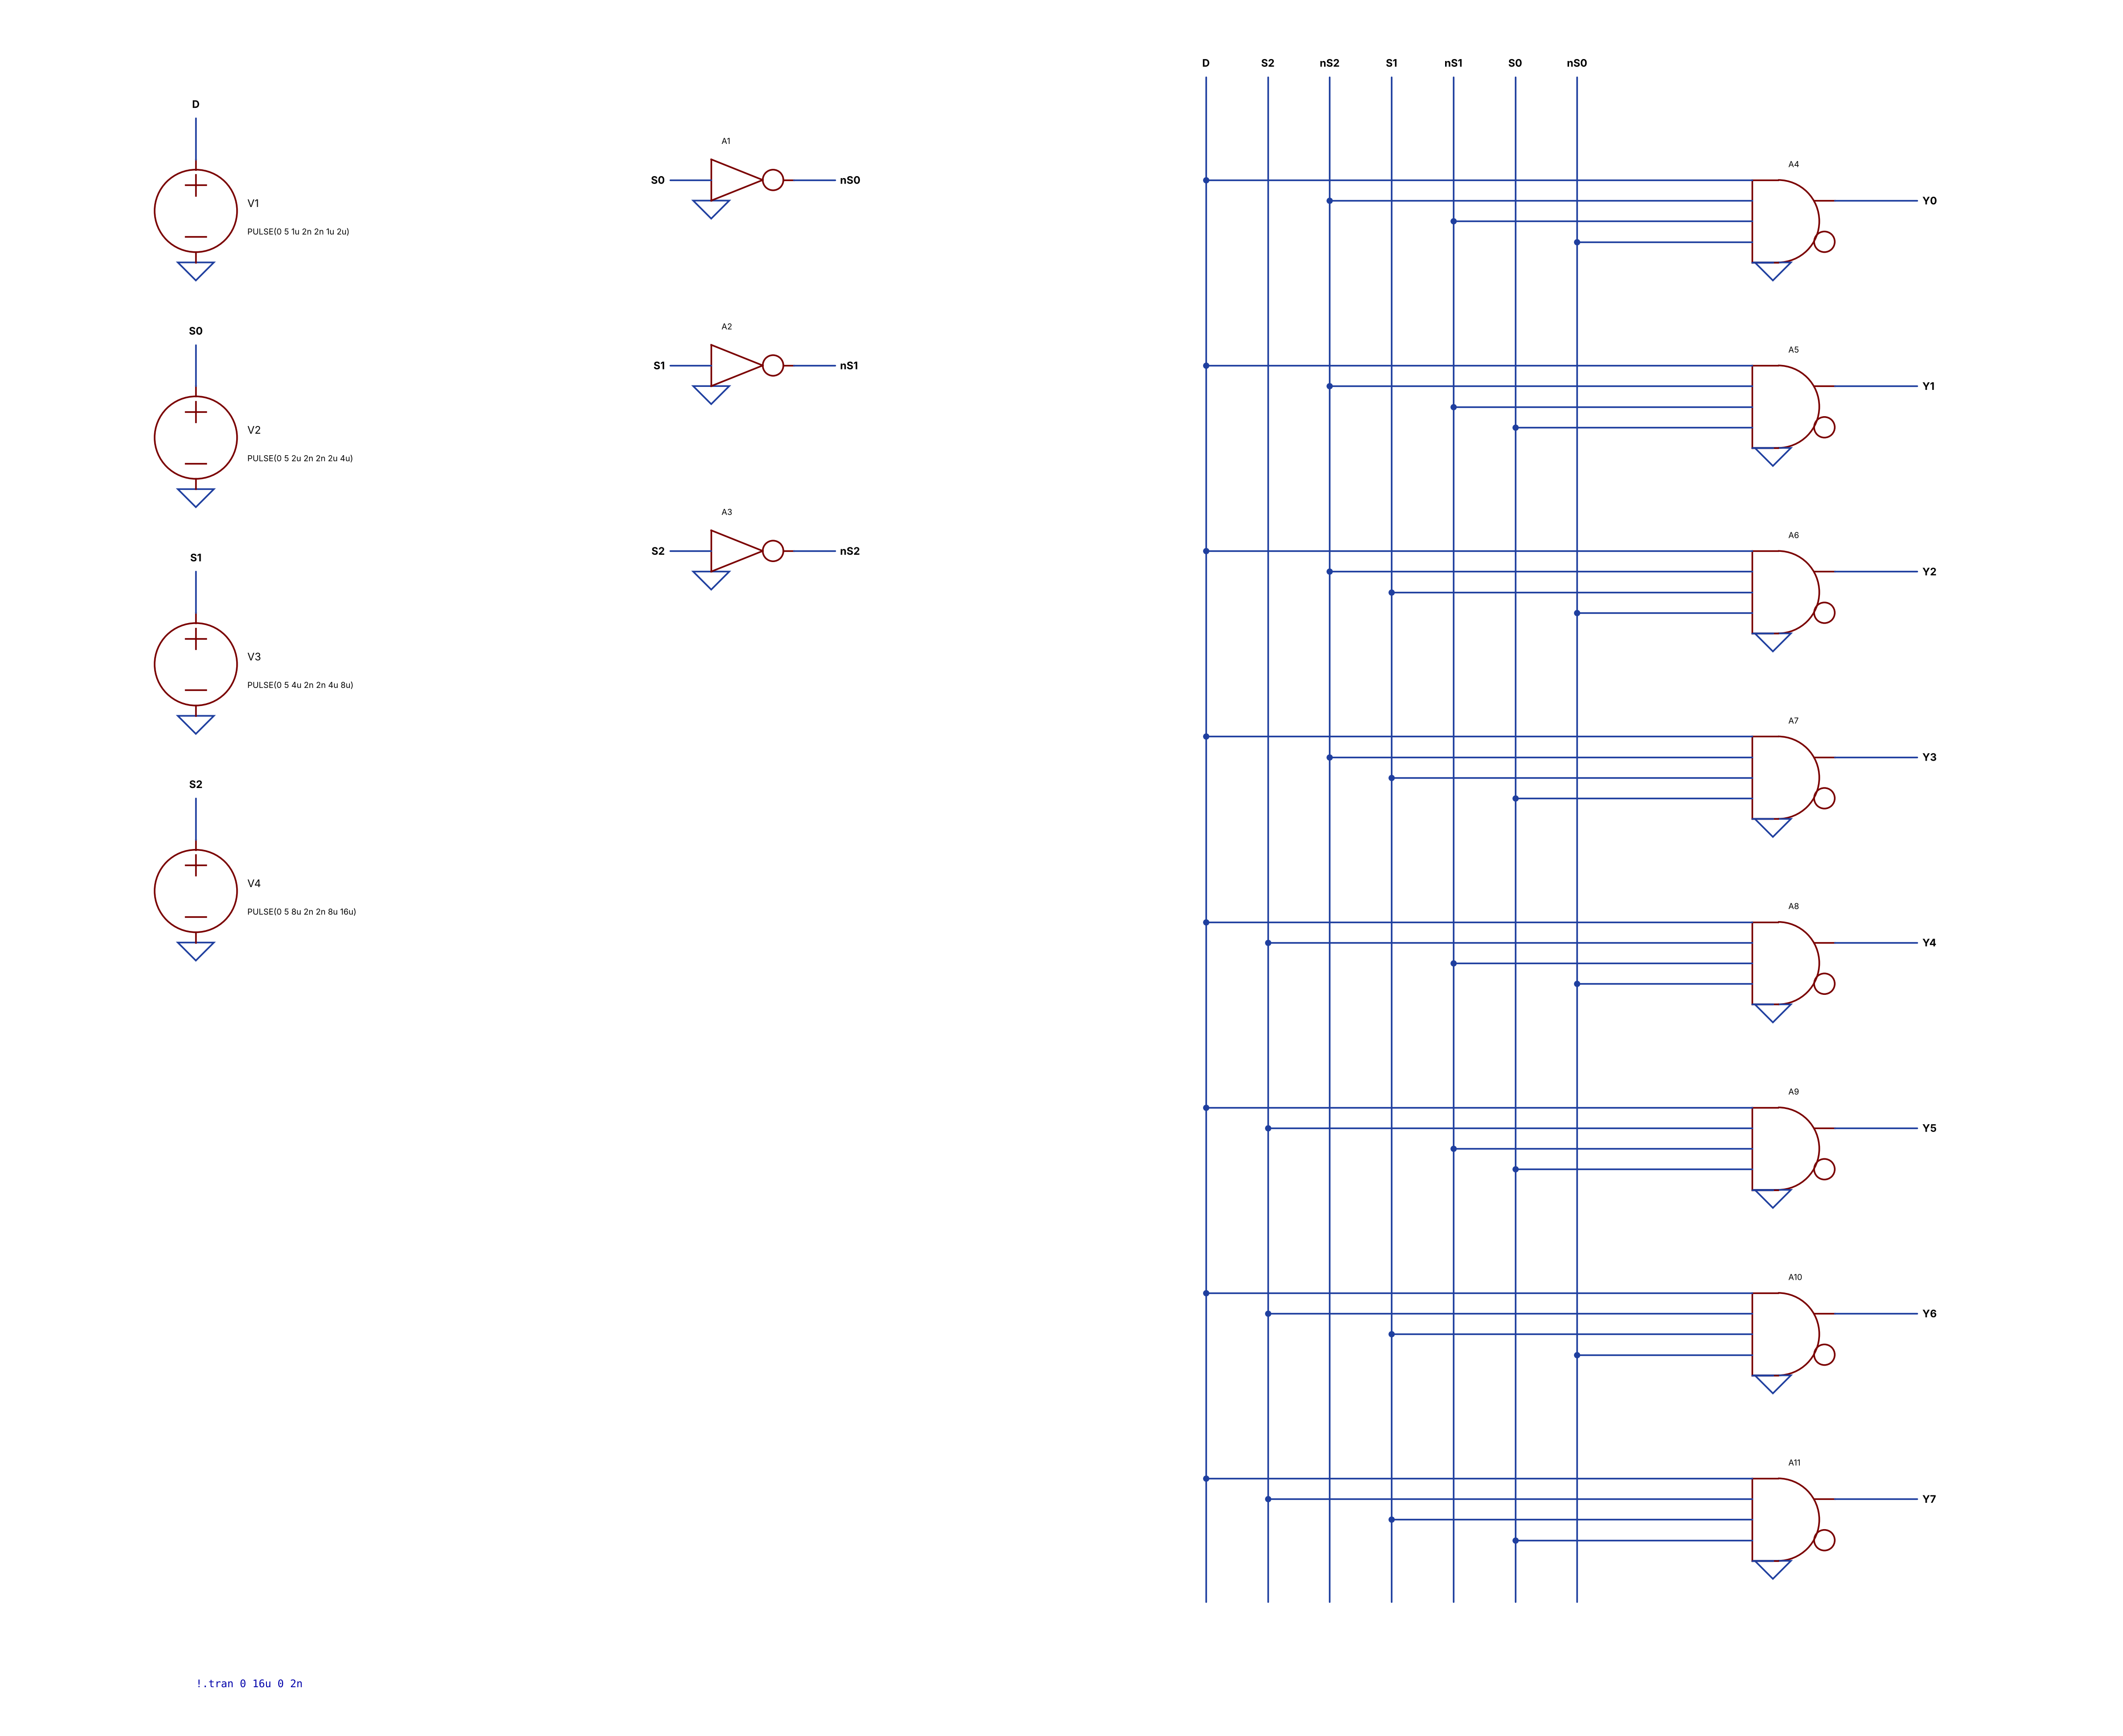
\includegraphics[width=\textwidth]{demux_1x8_sch.png}
\caption{Схема демультиплексора 1-в-8 в LTspice (файл \texttt{demux\_1x8.asc})}
\label{fig:demux_sch}
\end{figure}

\subsection{Входные сигналы}
\begin{itemize}
\item $D$: \texttt{PULSE(0 5 1u 2n 2n 1u 2u)} -- младший разряд перебора;
\item $S_0$: \texttt{PULSE(0 5 2u 2n 2n 2u 4u)};
\item $S_1$: \texttt{PULSE(0 5 4u 2n 2n 4u 8u)};
\item $S_2$: \texttt{PULSE(0 5 8u 2n 2n 8u 16u)};
\item директива \texttt{.tran 0 16u 0 2n} -- 16 комбинаций по 1 мкс.
\end{itemize}

\subsection{Результаты моделирования}
\begin{figure}[H]
\centering
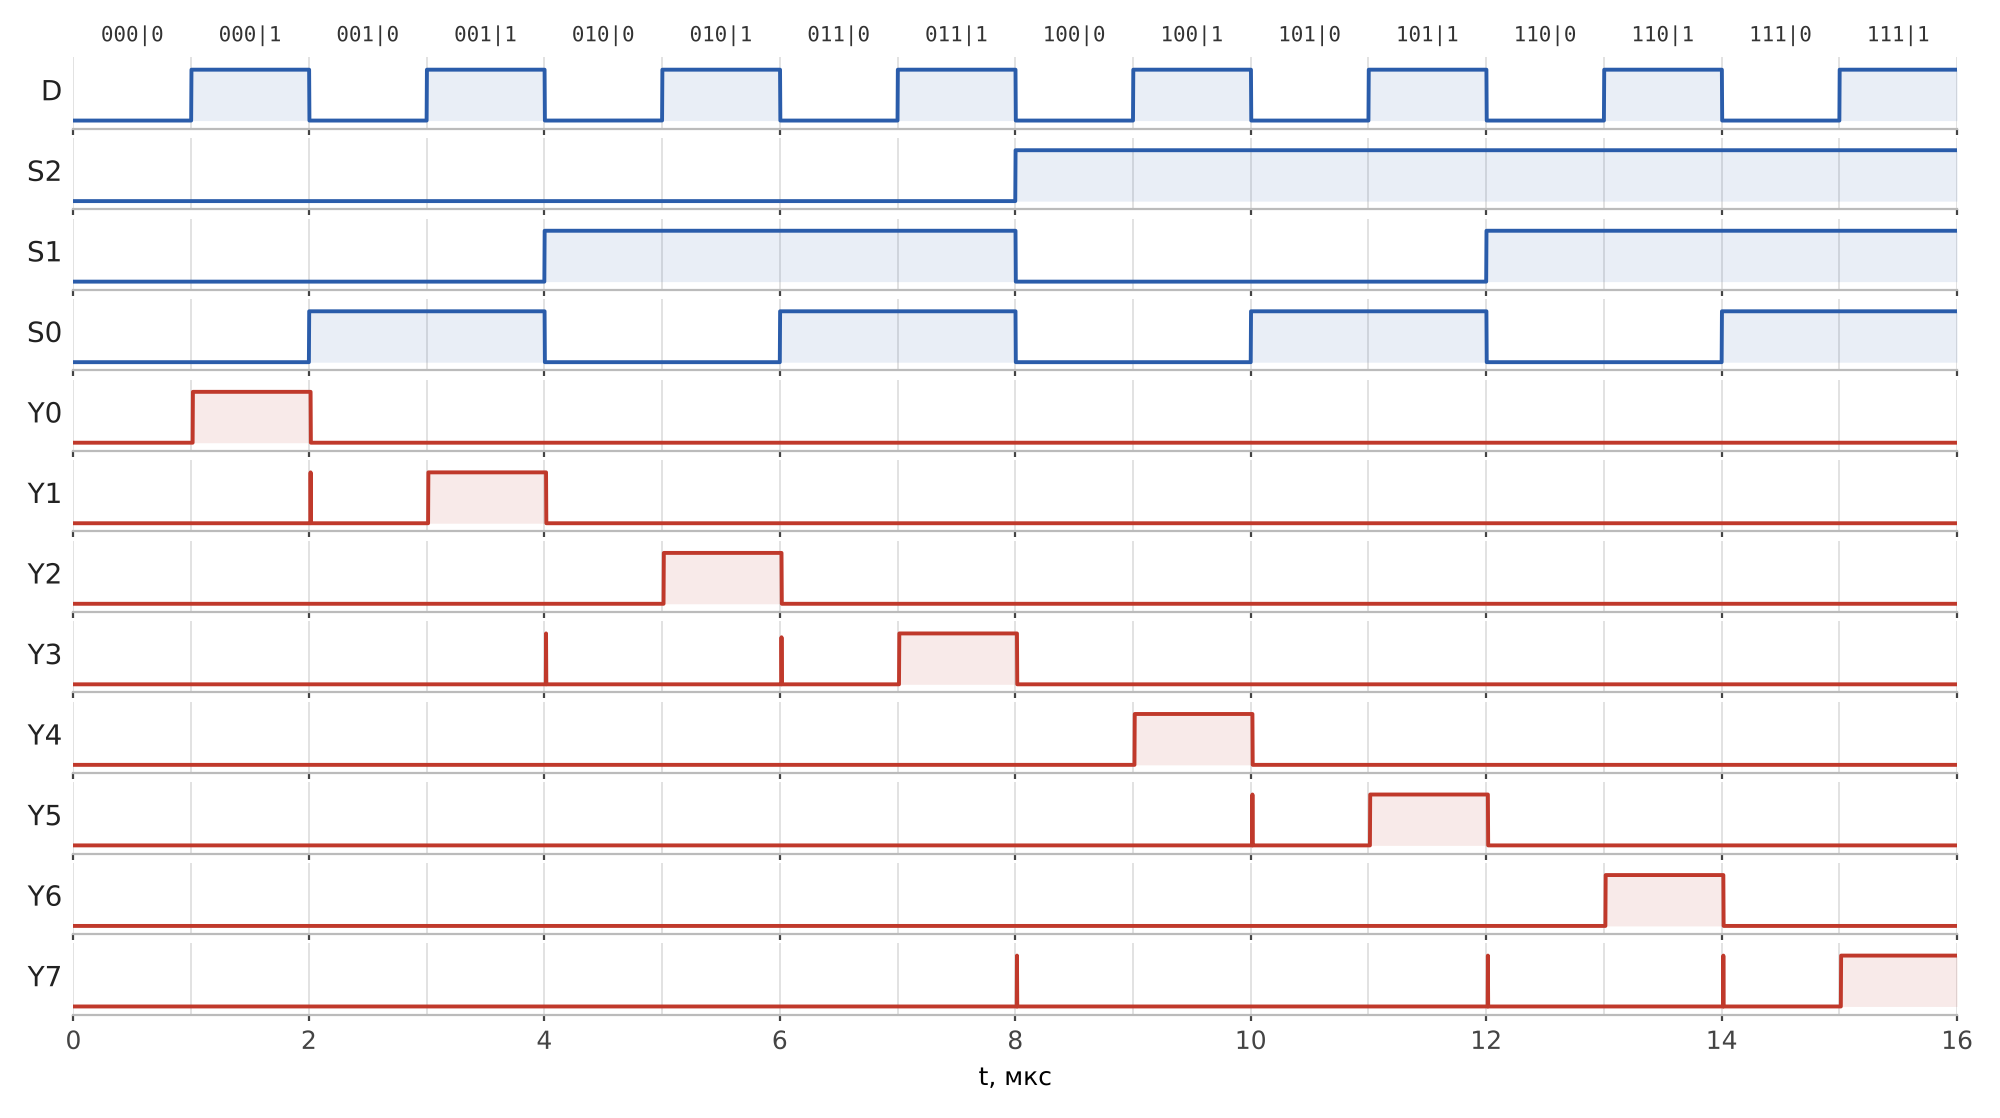
\includegraphics[width=\textwidth]{demux_1x8_wave.png}
\caption{Временные диаграммы демультиплексора 1-в-8. Над диаграммой указана текущая
комбинация в виде $S_2S_1S_0|D$}
\label{fig:demux_wave}
\end{figure}

По осциллограммам (значения считывались в середине каждого интервала) составлена таблица
истинности (табл.~\ref{tab:demux}).

\begin{table}[H]
\caption{Таблица истинности демультиплексора 1-в-8 по результатам моделирования}
\label{tab:demux}
\centering\small
\begin{tabular}{cccc|cccccccc|c}
\toprule
$D$ & $S_2$ & $S_1$ & $S_0$ & $Y_0$ & $Y_1$ & $Y_2$ & $Y_3$ & $Y_4$ & $Y_5$ & $Y_6$ & $Y_7$ & Теор. \\
\midrule
0 & 0 & 0 & 0 & 0 & 0 & 0 & 0 & 0 & 0 & 0 & 0 & \checkmark \\
0 & 0 & 0 & 1 & 0 & 0 & 0 & 0 & 0 & 0 & 0 & 0 & \checkmark \\
0 & 0 & 1 & 0 & 0 & 0 & 0 & 0 & 0 & 0 & 0 & 0 & \checkmark \\
0 & 0 & 1 & 1 & 0 & 0 & 0 & 0 & 0 & 0 & 0 & 0 & \checkmark \\
0 & 1 & 0 & 0 & 0 & 0 & 0 & 0 & 0 & 0 & 0 & 0 & \checkmark \\
0 & 1 & 0 & 1 & 0 & 0 & 0 & 0 & 0 & 0 & 0 & 0 & \checkmark \\
0 & 1 & 1 & 0 & 0 & 0 & 0 & 0 & 0 & 0 & 0 & 0 & \checkmark \\
0 & 1 & 1 & 1 & 0 & 0 & 0 & 0 & 0 & 0 & 0 & 0 & \checkmark \\
\midrule
1 & 0 & 0 & 0 & \textbf{1} & 0 & 0 & 0 & 0 & 0 & 0 & 0 & \checkmark \\
1 & 0 & 0 & 1 & 0 & \textbf{1} & 0 & 0 & 0 & 0 & 0 & 0 & \checkmark \\
1 & 0 & 1 & 0 & 0 & 0 & \textbf{1} & 0 & 0 & 0 & 0 & 0 & \checkmark \\
1 & 0 & 1 & 1 & 0 & 0 & 0 & \textbf{1} & 0 & 0 & 0 & 0 & \checkmark \\
1 & 1 & 0 & 0 & 0 & 0 & 0 & 0 & \textbf{1} & 0 & 0 & 0 & \checkmark \\
1 & 1 & 0 & 1 & 0 & 0 & 0 & 0 & 0 & \textbf{1} & 0 & 0 & \checkmark \\
1 & 1 & 1 & 0 & 0 & 0 & 0 & 0 & 0 & 0 & \textbf{1} & 0 & \checkmark \\
1 & 1 & 1 & 1 & 0 & 0 & 0 & 0 & 0 & 0 & 0 & \textbf{1} & \checkmark \\
\bottomrule
\end{tabular}
\end{table}

При $D=0$ все выходы равны нулю независимо от адреса, при $D=1$ активен ровно один выход
с номером $4S_2+2S_1+S_0$. Все 16 строк совпадают с теоретической таблицей.

\subsection{Анализ переходных процессов}
На рис.~\ref{fig:demux_wave} на выходах $Y_1$, $Y_3$, $Y_5$, $Y_7$ видны короткие
ложные импульсы (глитчи) в моменты 2, 4, 6, 8, 10, 12 и 14~мкс. Их длительность около
2~нс (рис.~\ref{fig:demux_zoom}). Причина -- состязание (гонка) входных сигналов:
у источника \texttt{PULSE} спад начинается в момент $t_d+t_r+PW$, т.\,е. на 2~нс позже
фронта источника, переключающегося «в тот же» момент. Например, в $t=4$~мкс сигнал $S_1$
уже стал равен 1, а $D$ и $S_0$ ещё не успели упасть, поэтому на 2~нс выполняется условие
$D\,\nm{S_2}\,S_1\,S_0=1$ и на $Y_3$ появляется импульс, задержанный на $t_d=10$~нс.
В реальной схеме такие глитчи возникают из-за неодинаковых задержек путей и устраняются
стробированием (разрешением выхода после установления адреса).

\begin{figure}[H]
\centering
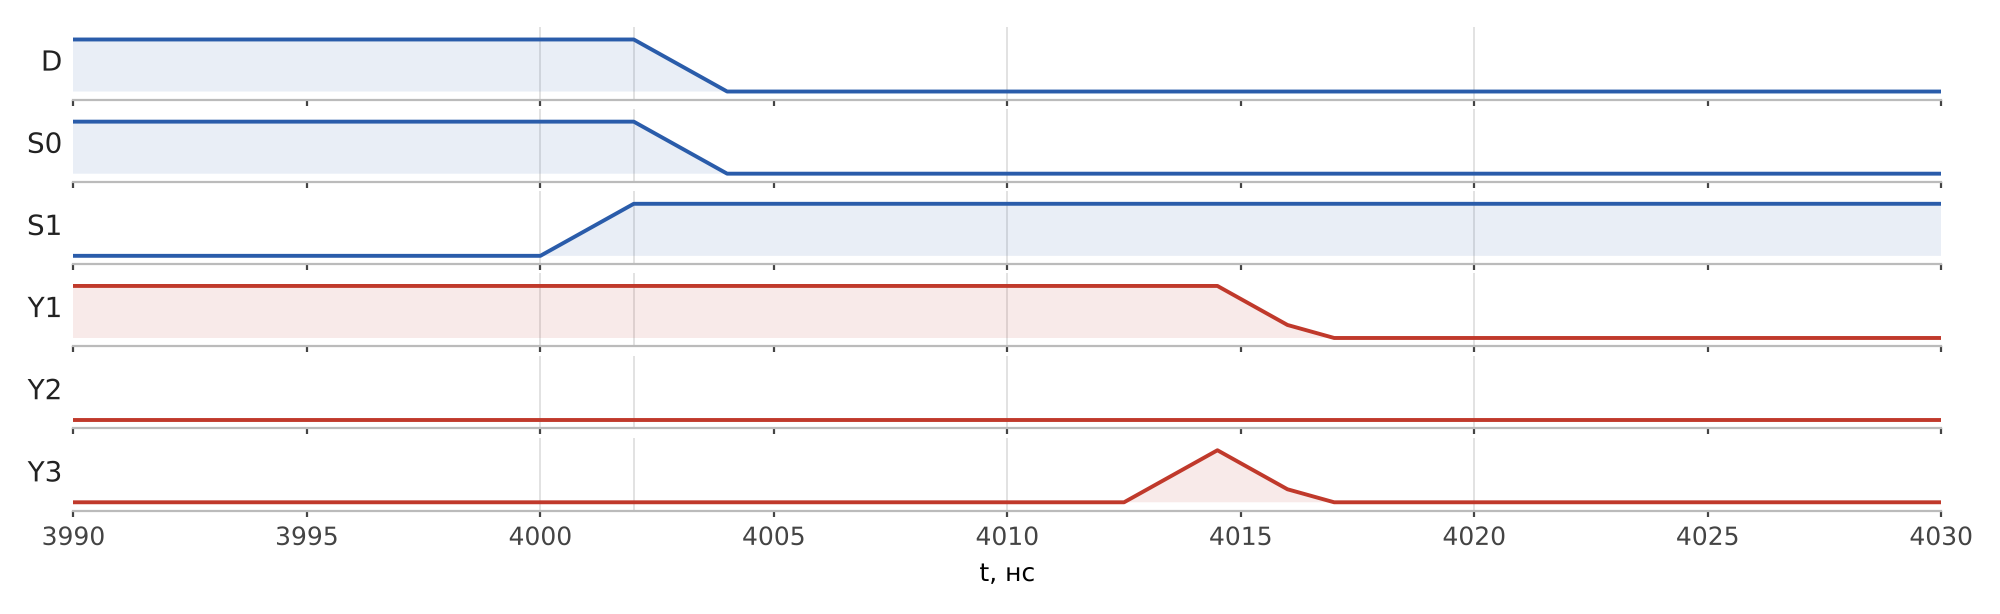
\includegraphics[width=0.9\textwidth]{demux_1x8_zoom.png}
\caption{Ложный импульс на выходе $Y_3$ при переключении адреса в $t=4$~мкс}
\label{fig:demux_zoom}
\end{figure}

% =====================================================================
\section{Шифратор 8-в-3}
\subsection{Принцип работы и структурная схема}
Шифратор преобразует номер активного входа $I_0\ldots I_7$ (унитарный код) в
трёхразрядный двоичный код $A_2A_1A_0$. Разряд $A_j$ равен единице, если активен вход,
в двоичном номере которого $j$-й разряд равен 1:
\begin{equation}
A_0 = I_1+I_3+I_5+I_7,\qquad
A_1 = I_2+I_3+I_6+I_7,\qquad
A_2 = I_4+I_5+I_6+I_7.
\end{equation}
Схема состоит из трёх четырёхвходовых элементов ИЛИ (рис.~\ref{fig:enc_sch}); вход $I_0$
в формировании кода не участвует, так как ему соответствует код 000.

\begin{figure}[H]
\centering
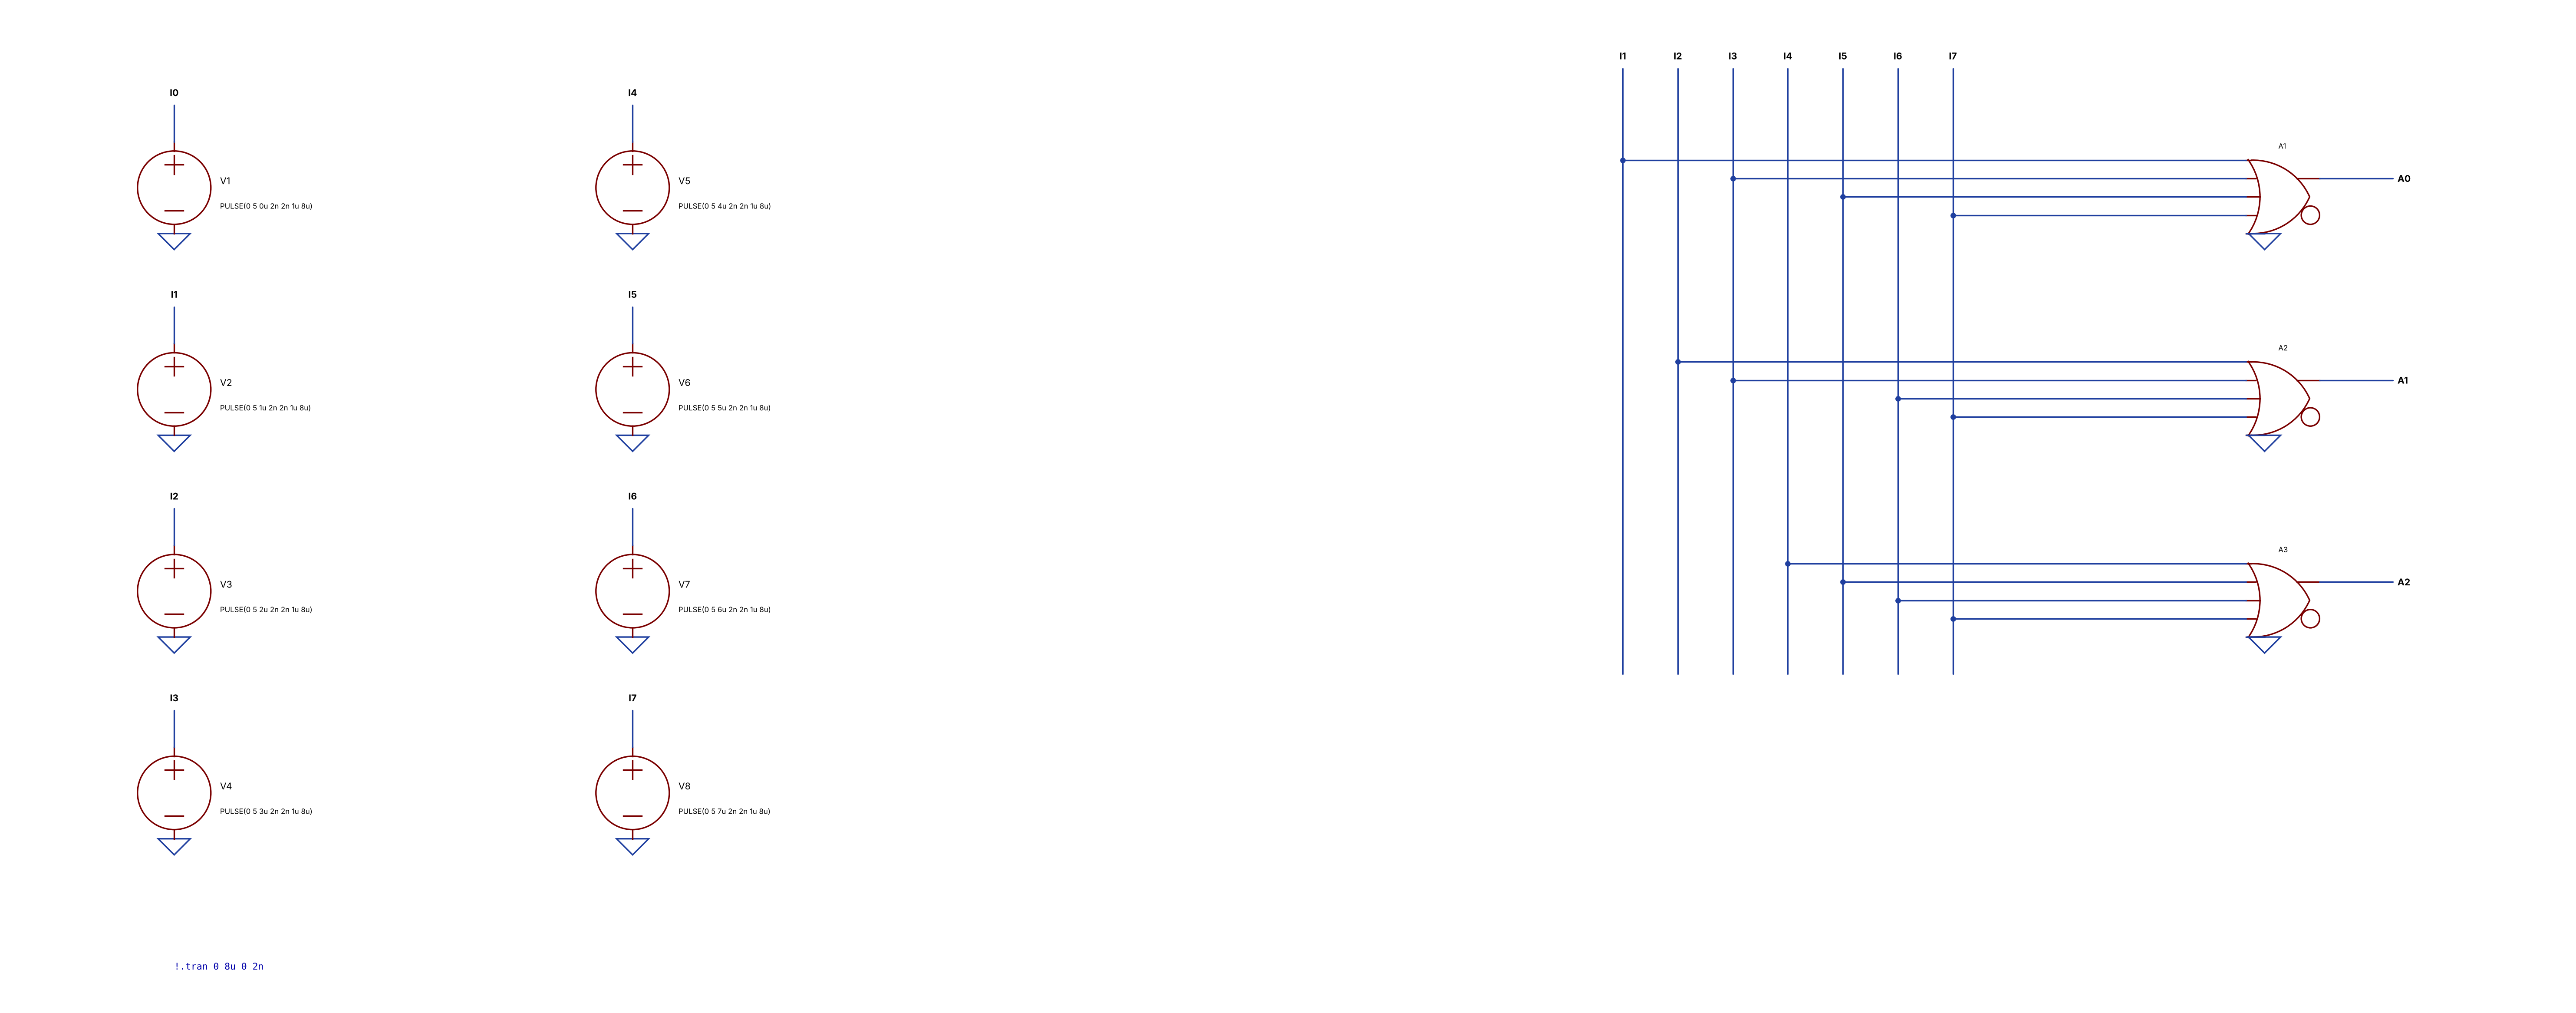
\includegraphics[width=\textwidth]{encoder_8x3_sch.png}
\caption{Схема шифратора 8-в-3 в LTspice (файл \texttt{encoder\_8x3.asc})}
\label{fig:enc_sch}
\end{figure}

\subsection{Входные сигналы}
Для шифратора допустимыми являются комбинации, в которых активен ровно один вход,
поэтому источники заданы как «бегущая единица»: источник $I_k$ --
\texttt{PULSE(0 5 $k$u 2n 2n 1u 8u)}, $k=0\ldots7$, директива \texttt{.tran 0 8u 0 2n}.

\subsection{Результаты моделирования}
\begin{figure}[H]
\centering
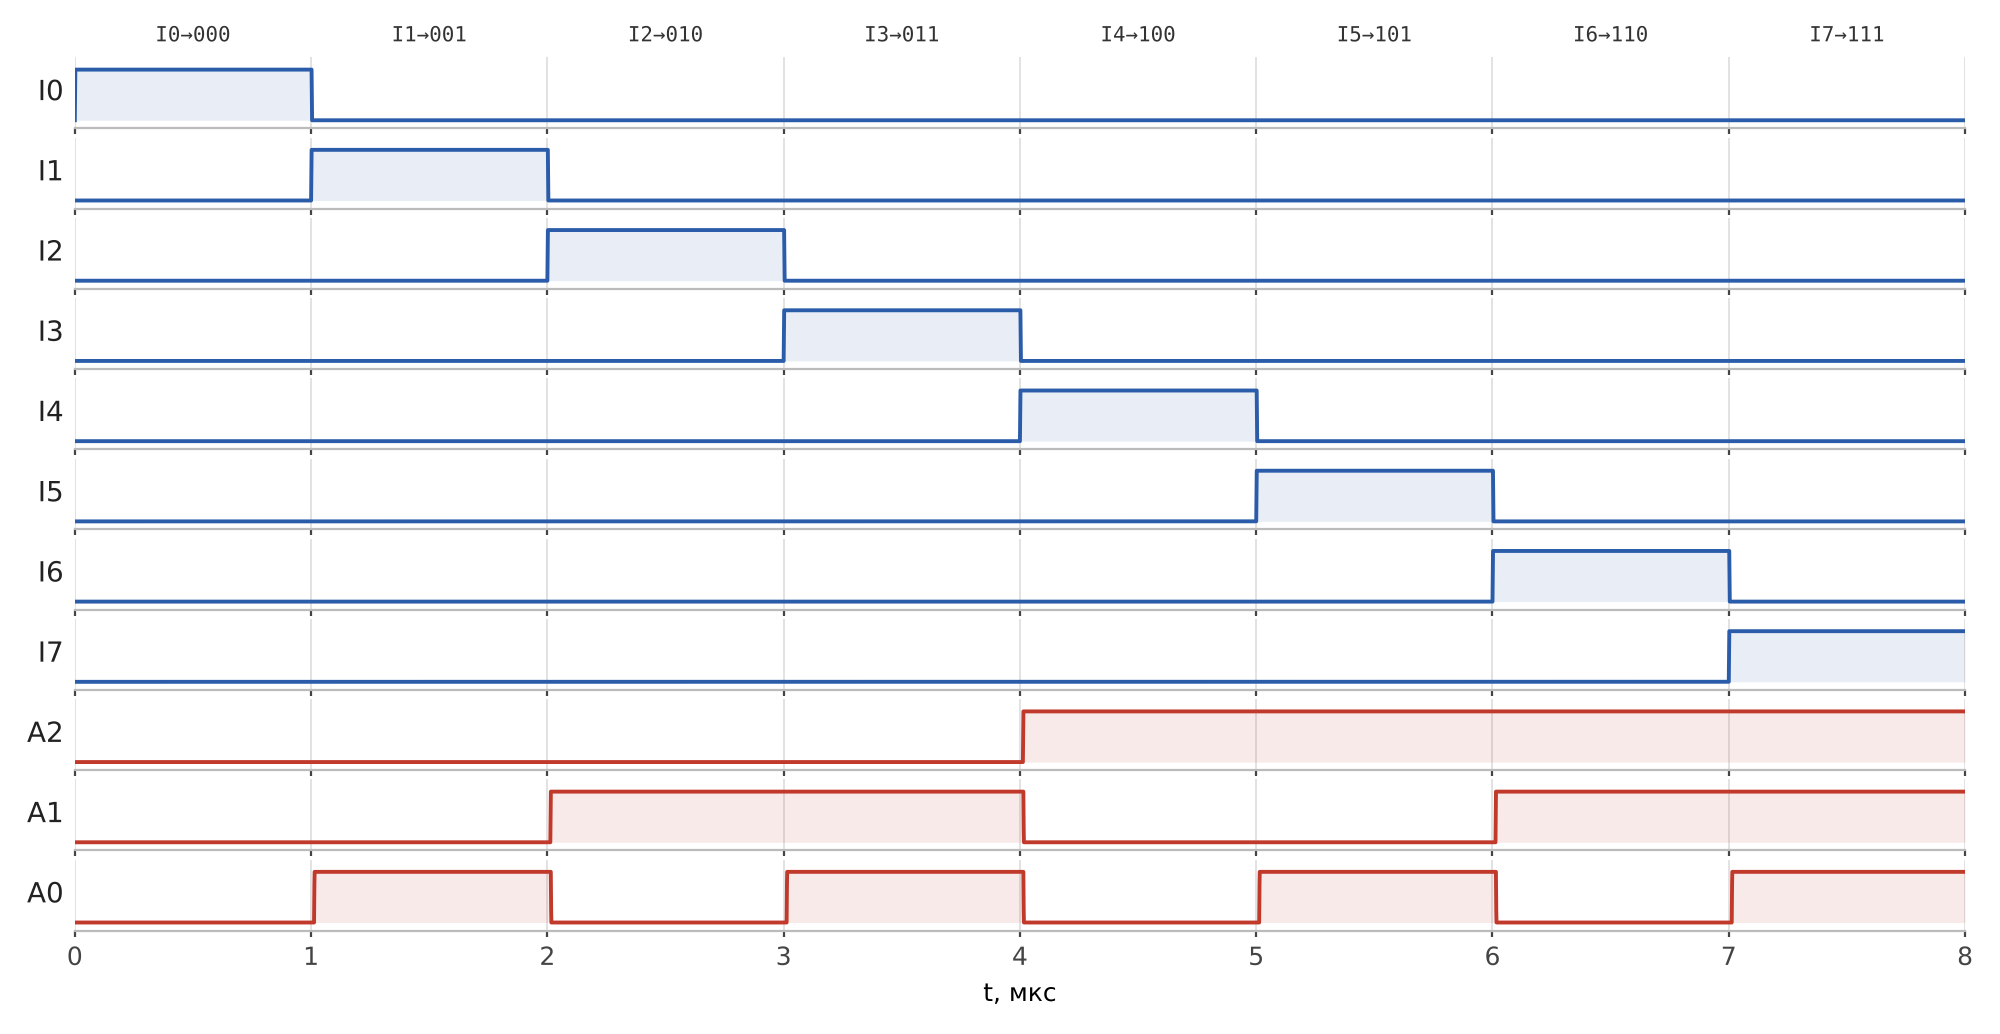
\includegraphics[width=\textwidth]{encoder_8x3_wave.png}
\caption{Временные диаграммы шифратора 8-в-3 (сверху -- активный вход и ожидаемый код)}
\label{fig:enc_wave}
\end{figure}

\begin{table}[H]
\caption{Таблица истинности шифратора 8-в-3 по результатам моделирования}
\label{tab:enc}
\centering\small
\begin{tabular}{cccccccc|ccc|c}
\toprule
$I_7$ & $I_6$ & $I_5$ & $I_4$ & $I_3$ & $I_2$ & $I_1$ & $I_0$ & $A_2$ & $A_1$ & $A_0$ & Теор. \\
\midrule
0 & 0 & 0 & 0 & 0 & 0 & 0 & \textbf{1} & 0 & 0 & 0 & \checkmark \\
0 & 0 & 0 & 0 & 0 & 0 & \textbf{1} & 0 & 0 & 0 & 1 & \checkmark \\
0 & 0 & 0 & 0 & 0 & \textbf{1} & 0 & 0 & 0 & 1 & 0 & \checkmark \\
0 & 0 & 0 & 0 & \textbf{1} & 0 & 0 & 0 & 0 & 1 & 1 & \checkmark \\
0 & 0 & 0 & \textbf{1} & 0 & 0 & 0 & 0 & 1 & 0 & 0 & \checkmark \\
0 & 0 & \textbf{1} & 0 & 0 & 0 & 0 & 0 & 1 & 0 & 1 & \checkmark \\
0 & \textbf{1} & 0 & 0 & 0 & 0 & 0 & 0 & 1 & 1 & 0 & \checkmark \\
\textbf{1} & 0 & 0 & 0 & 0 & 0 & 0 & 0 & 1 & 1 & 1 & \checkmark \\
\bottomrule
\end{tabular}
\end{table}

Выходной код во всех восьми случаях совпадает с двоичным номером активного входа.

\subsection{Анализ}
Все выходы переключаются одновременно с задержкой $t_d\approx10$~нс (один уровень логики),
поэтому глитчей не наблюдается. Особенности простого шифратора, следующие из уравнений (2):
\begin{itemize}
\item отсутствие активных входов и активный вход $I_0$ дают одинаковый код 000, поэтому
на практике добавляют выход признака «есть активный вход»;
\item при одновременной активности нескольких входов на выходе получается поразрядное ИЛИ
их кодов (например, $I_3$ и $I_4$ дают $011+100=111$), то есть ложный номер. Для таких
случаев используют приоритетный шифратор.
\end{itemize}

% =====================================================================
\section{Полный сумматор}
\subsection{Принцип работы и структурная схема}
Полный сумматор складывает три одноразрядных числа: $A$, $B$ и перенос из младшего
разряда $C_{in}$, формируя сумму $S$ и перенос в старший разряд $C_{out}$:
\begin{equation}
S = A\oplus B\oplus C_{in},\qquad C_{out}=A\,B + C_{in}\,(A\oplus B).
\end{equation}
Схема построена из двух полусумматоров и элемента ИЛИ (рис.~\ref{fig:fa_sch}):
$P=A\oplus B$, $G=A\,B$, $S=P\oplus C_{in}$, $K=P\,C_{in}$, $C_{out}=G+K$.

\begin{figure}[H]
\centering
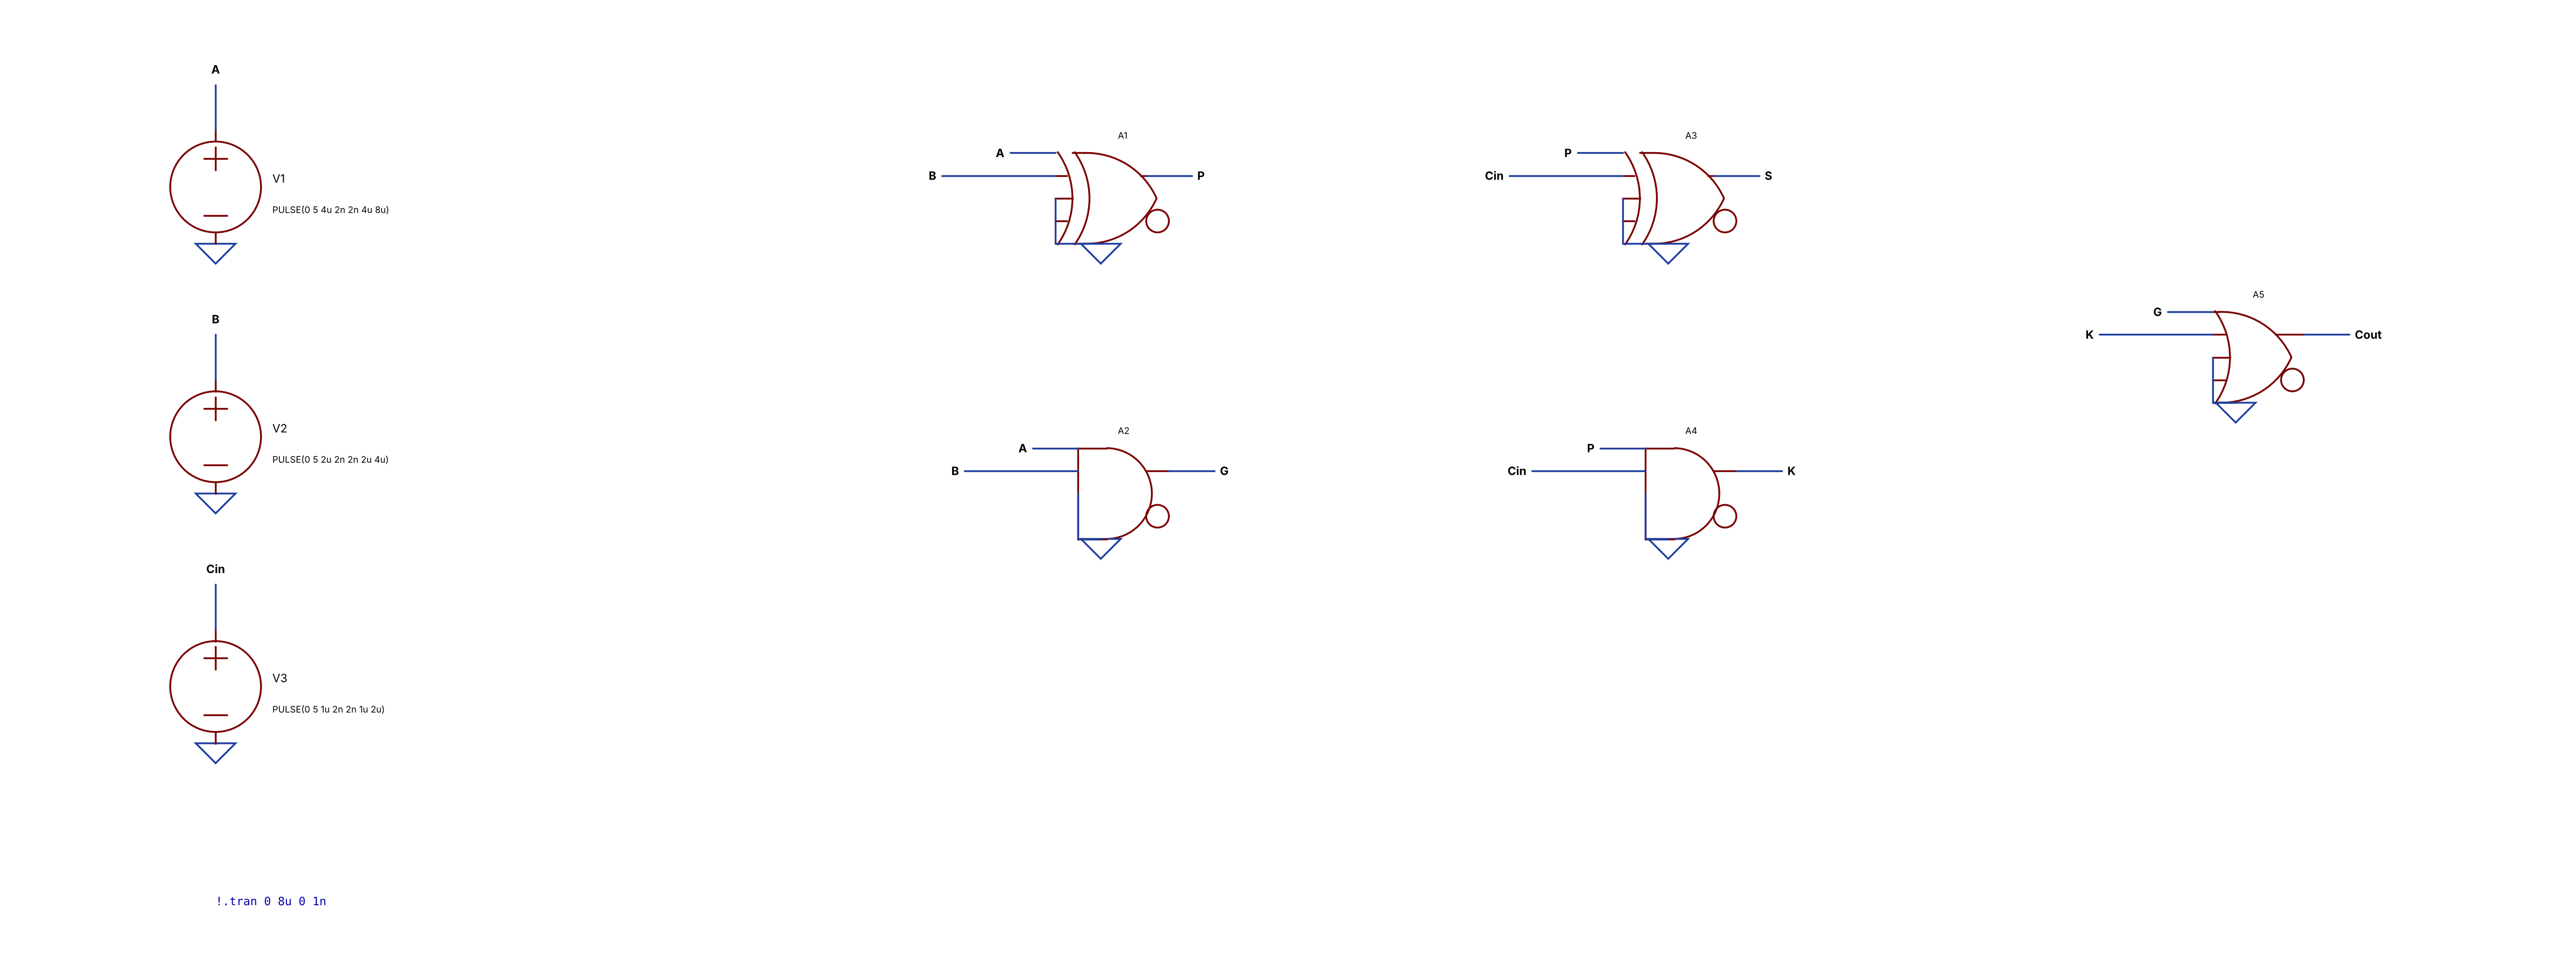
\includegraphics[width=\textwidth]{full_adder_sch.png}
\caption{Схема полного сумматора в LTspice (файл \texttt{full\_adder.asc})}
\label{fig:fa_sch}
\end{figure}

\subsection{Входные сигналы}
$C_{in}$: \texttt{PULSE(0 5 1u 2n 2n 1u 2u)}, $B$: \texttt{PULSE(0 5 2u 2n 2n 2u 4u)},
$A$: \texttt{PULSE(0 5 4u 2n 2n 4u 8u)}, директива \texttt{.tran 0 8u 0 1n} --
8 комбинаций $ABC_{in}$ от 000 до 111.

\subsection{Результаты моделирования}
\begin{figure}[H]
\centering
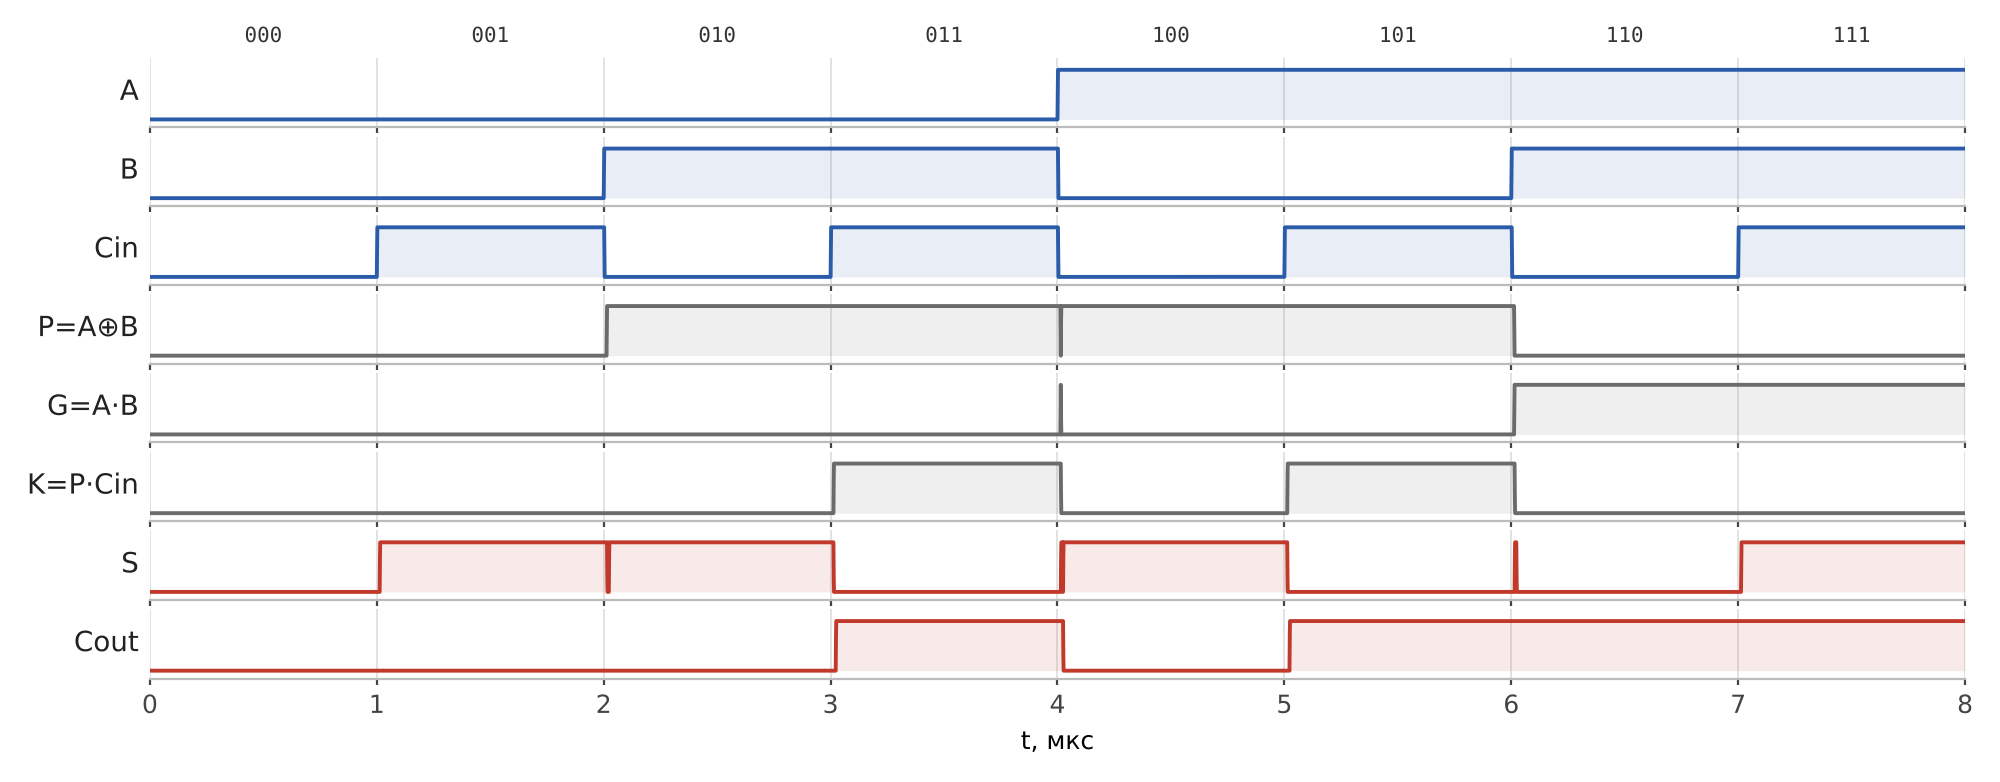
\includegraphics[width=\textwidth]{full_adder_wave.png}
\caption{Временные диаграммы полного сумматора (сверху -- комбинация $A\,B\,C_{in}$)}
\label{fig:fa_wave}
\end{figure}

\begin{table}[H]
\caption{Таблица истинности полного сумматора по результатам моделирования}
\label{tab:fa}
\centering
\begin{tabular}{ccc|cc|c|c}
\toprule
$A$ & $B$ & $C_{in}$ & $S$ & $C_{out}$ & $A+B+C_{in}$ & Теор. \\
\midrule
0 & 0 & 0 & 0 & 0 & 0 = $(00)_2$ & \checkmark \\
0 & 0 & 1 & 1 & 0 & 1 = $(01)_2$ & \checkmark \\
0 & 1 & 0 & 1 & 0 & 1 = $(01)_2$ & \checkmark \\
0 & 1 & 1 & 0 & 1 & 2 = $(10)_2$ & \checkmark \\
1 & 0 & 0 & 1 & 0 & 1 = $(01)_2$ & \checkmark \\
1 & 0 & 1 & 0 & 1 & 2 = $(10)_2$ & \checkmark \\
1 & 1 & 0 & 0 & 1 & 2 = $(10)_2$ & \checkmark \\
1 & 1 & 1 & 1 & 1 & 3 = $(11)_2$ & \checkmark \\
\bottomrule
\end{tabular}
\end{table}

Во всех восьми случаях двоичное число $C_{out}S$ равно арифметической сумме
$A+B+C_{in}$, что соответствует теоретической таблице.

\subsection{Анализ переходных процессов}
Сигналы проходят до выходов через разное число элементов: путь
$C_{in}\to S$ содержит один элемент XOR, путь $A,B\to P\to S$ -- два. Поэтому при
одновременном изменении $C_{in}$ и $B$ (моменты 2, 4 и 6~мкс) выход $S$ сначала реагирует
на изменение $C_{in}$, а через $t_d$ -- на изменение $P$. Например, в $t=2$~мкс
комбинация меняется $001\to010$, теоретически $S$ должен оставаться равным 1, но на
диаграмме виден провал длительностью около 8~нс (рис.~\ref{fig:fa_zoom}) -- статический
риск сбоя (hazard). В момент 4~мкс ($011\to100$) кроме этого виден ещё один короткий
импульс шириной около 2~нс, вызванный разнесением фронтов источников.
Выход $C_{out}$ в данном опыте ложных переключений не показал. Установившиеся значения
всегда правильные, поэтому в синхронных схемах такие кратковременные сбои не опасны,
если выход считывается после окончания переходного процесса (задержка не более
$2t_d=20$~нс для $S$ и $3t_d=30$~нс для $C_{out}$).

\begin{figure}[H]
\centering
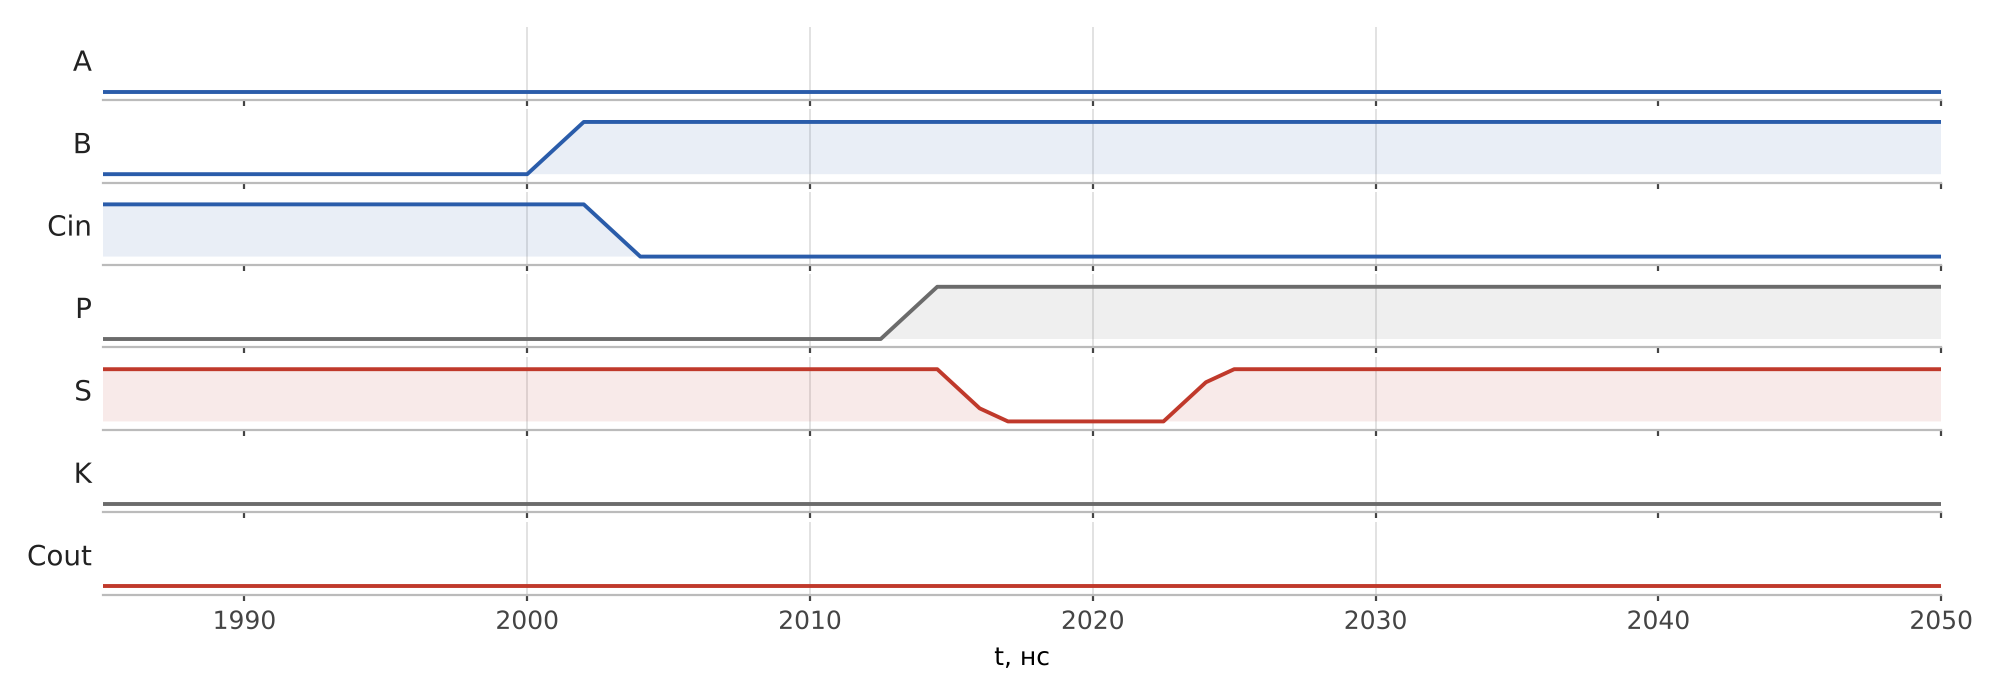
\includegraphics[width=0.9\textwidth]{full_adder_zoom.png}
\caption{Статический риск сбоя на выходе $S$ при переходе $001\to010$ ($t=2$~мкс)}
\label{fig:fa_zoom}
\end{figure}

% =====================================================================
\section{Сравнение теоретических и полученных результатов}
\begin{table}[H]
\caption{Сводка результатов}\label{tab:sum}
\centering\small
\begin{tabular}{p{3.6cm}p{3.6cm}p{7.6cm}}
\toprule
Схема & Таблица истинности & Отличия и аномалии переходов\\
\midrule
Демультиплексор 1-в-8 & 16/16 совпадений & глитчи ~2 нс на $Y_1,Y_3,Y_5,Y_7$ при одновременной
смене нескольких входов; задержка $t_d$ (1 уровень И) + $t_d$ инвертора\\
Шифратор 8-в-3 & 8/8 совпадений & задержка $t_d$, глитчей нет; неоднозначность кода 000\\
Полный сумматор & 8/8 совпадений & риск сбоя на $S$ (~8 нс) из-за разной длины путей;
задержка до $2t_d$ ($S$) и $3t_d$ ($C_{out}$)\\
\bottomrule
\end{tabular}
\end{table}

% =====================================================================
\section{Ответы на контрольные вопросы}
\textbf{1. В чём разница между мультиплексором и дешифратором?}
Мультиплексор имеет $2^n$ информационных входов, $n$ адресных входов и один выход: он
передаёт на выход значение выбранного входа. Дешифратор имеет $n$ входов кода и $2^n$
выходов: он активирует выход, номер которого равен входному коду, и информационных входов
не имеет (кроме входа разрешения). Внутри мультиплексора, по сути, стоит дешифратор адреса,
выходы которого стробируют информационные входы.

\textbf{2. Как реализовать 4-в-1 мультиплексор на базовых логических элементах?}
По уравнению $Y=\nm{S_1}\,\nm{S_0}\,I_0+\nm{S_1}\,S_0\,I_1+S_1\,\nm{S_0}\,I_2+S_1\,S_0\,I_3$:
два инвертора для $\nm{S_1},\nm{S_0}$, четыре трёхвходовых элемента И и один
четырёхвходовый элемент ИЛИ.

\textbf{3. Как работает полный сумматор и чем он отличается от полусумматора?}
Полусумматор складывает два бита: $S=A\oplus B$, $C=A\,B$, и не учитывает перенос из младшего
разряда. Полный сумматор имеет третий вход $C_{in}$ и вычисляет $S=A\oplus B\oplus C_{in}$,
$C_{out}=AB+C_{in}(A\oplus B)$; его можно собрать из двух полусумматоров и элемента ИЛИ, и
он позволяет каскадно строить многоразрядные сумматоры.

\textbf{4. Почему дешифратор не используется для прямого хранения состояния?}
Дешифратор -- комбинационная схема без обратных связей: его выходы однозначно определяются
текущими входами и сразу (через время задержки) меняются вслед за ними. Элементов памяти в
нём нет, поэтому после снятия входного кода информация теряется. Для хранения нужны
последовательностные схемы -- триггеры и регистры.

\textbf{5. Как связаны шифратор и дешифратор по логике работы?}
Это взаимно обратные преобразования: шифратор переводит унитарный код («один из $2^n$») в
$n$-разрядный двоичный, а дешифратор -- двоичный код в унитарный. Последовательное
включение дешифратора и шифратора восстанавливает исходный код.

% =====================================================================
\section*{Выводы}
\addcontentsline{toc}{section}{Выводы}
\begin{enumerate}[leftmargin=*, label=\arabic*.]
\item В LTspice собраны на базовых логических элементах три комбинационные схемы варианта 2:
демультиплексор 1-в-8 (3 инвертора + 8 элементов И), шифратор 8-в-3 (3 элемента ИЛИ) и
полный сумматор (2 XOR, 2 И, 1 ИЛИ).
\item Подачей сигналов \texttt{PULSE} с кратными периодами перебраны все входные
комбинации; построенные по осциллограммам таблицы истинности полностью совпали с
теоретическими (16, 8 и 8 строк соответственно).
\item Выходы комбинационных схем зависят только от текущих входов и устанавливаются с
задержкой, пропорциональной числу уровней логики (10--30~нс при $t_d=10$~нс).
\item Во время переходов зафиксированы кратковременные ложные импульсы: у демультиплексора
-- из-за неодновременного переключения входов, у сумматора -- из-за разной длины путей
распространения сигнала (риск сбоя). На установившиеся значения они не влияют, но их нужно
учитывать при асинхронном использовании выходов.
\item Простой шифратор корректен только при одном активном входе; для произвольных
комбинаций требуется приоритетный шифратор.
\end{enumerate}

\section*{Список литературы}
\addcontentsline{toc}{section}{Список литературы}
\begin{enumerate}[leftmargin=*, label=\arabic*.]
\item Хоровиц П., Хилл У. Искусство схемотехники / Пер. с англ. Изд. 2-е. -- М.: БИНОМ, 2014. -- 740 с.
\item Бойко В.\,И. Схемотехника электронных систем. Аналоговые и импульсные устройства. -- 2004.
\end{enumerate}

\end{document}
